\chapter{Evaluation in Test Domains}
\thispagestyle{plain}

\label{ch:evaluation}
This chapter presents the results of applying the algorithms described in the previous chapter to three test domains.  I show that, in many cases, the utility loss from PS Map approximation is comparable to that of online repair.  However, the performance of the approximation algorithms varies between problem domains and between different problem configurations within the same problem domain.  In both cases, the differences in the size and quantity of heterogeneous regions intrinsic to the problem domain and configuration appear to be suggestive as reasons for the differences in approximation accuracy.  I tested the algorithms using the traveling saleman problem (TSP), the knapsack problem, and an elevator problem.  The TSP and knapsack problems are classic domains in optimization and computer science.  The elevator problem is a challenge domain created for the AAAI International Planning Competition (IPC) \citep{coles2013survey}.  All of the problems are NP-complete or NP-hard, and quickly become intractable with complex enough problem instances.



Traditional TSP problems consist of a set of unordered locations, sometimes referred to as ``cities,'' that must be ordered such that the length of route that traverses the set is minimized.  In the dynamic variant, one or more additional locations become known after the initial ordering is computed, and must be incorporated into the route while minimizing computation time and total route distance.

In the knapsack problem, one chooses from a set  of given items, each with a weight and value characteristic, such that the total value of the knapsack is maximized and the total weight does not exceed a given weight constraint.  I use the 0-1 variant, in which each item may  be selected a maximum of one time.  After computing an initial solution, I present one or more  additional items with which the system may revise its solution.

The elevator domain defines the initial and desired locations of a set of  passengers, and several elevators of varying speeds with which to transport passengers.  The goal is to move all the passengers to their desired floors as cheaply as possible through efficient use of elevator movements.  For my testing, I use a variant in which one or more passengers' initial location may change after the initial plan is computed.

My primary metric for evaluation is utility loss, measured as a fraction of the utility of a problem instance's high-quality\footnote{As previously mentioned, ``high-quality'' refers to solutions generated by heuristic search methods.  As solutions to intractable problems they cannot be guaranteed to be optimal; therefore, I avoid the use of that term.} solution, as calculated by a heuristic solver.  For example, if the total value of a high-quality knapsack solution is 100, and the solution retrieved from the approximated PS Map has a value of 95, then the utility loss for that specific solution is .05 (i.e., $\frac{100-95}{100}$).  The evaluation of an approximated PS Map is the average utility loss over all of the discrete locations in the map.  Thus, the evaluation for a PS Map over all problem instances is $\frac{\sum_{i \in map}heuristic_i-approx_i}{\sum_{i \in map}heuristic_i}$ where $approx_i$ and $heuristic_i$ are the utility of the solutions given by the PS Map and a heuristic planner, respectively, for a given problem instance $i$.  Lower utility loss is preferred; the best approximated solution will have a utility loss of zero.


\section{Traveling Salesman Problem}

The traveling salesman problem (TSP) is a classic NP-complete problem in computer science in which cities must be ordered such that the length of the resulting route is minimized.  The dynamic variant, the DTSP, allows for cities to be removed or added while the route is being traversed, creating a more challenging problem in which the route should be reoptimized in real time.  I used the TSP as an initial domain for algorithm validation and development.  I generated problem instances ranging from 5 cities to 100 cities, representing a range of problem complexity.  The algorithms were developed based upon the insights from tests of  each preceding algorithm, which will be reflected in some of the discussion.  In addition to the inter-algorithm comparison, I also generated baseline results from typical online repair techniques.

\subsection{High-Quality PS Map} For testing in the TSP domain, I generated three instances each of 5, 10, 20, 50, and 100-city DTSPs.  One of the cities included with each of the DTSPs has a  variable location.  As the gold standard, high-quality PS Maps were generated via the Clark-Wright \citep{clarke64scheduling} and Gillett-Miller \citep{gillett74heuristic} algorithms, as implemented by the Drasys library.\footnote{As of this writing, this library appears to no longer be publicly available.  I have placed a copy of the original download at  \url{http://www.umbc.edu/~holder1/or124.jar}}  I then removed errors stemming from heuristic-based solvers by executing the SSS algorithm over the PS Map.  As described in Section \ref{sec:sss}, this process tests each unique solution against each problem instance, resulting in a more accurate PS Map.  


\subsection{Online Repair Baseline} To compare how well PS Map approximation techniques perform against traditional online repair, I implemented the insertion approach \citep{psaraftis88dynamic}.  This approach incorporates new cities into the route by finding the nearest city and inserting the new city into the route either before or after the nearest city.  Although it is not the best repair technique, it is well suited for online repair due to its speed.  In this case, the repair accuracy was within the expected loss of utility provided by other  DTSP online repair algorithms as discussed by \citeauthor{larsen2000dvrp}.  This baseline will be discussed in more detail when presenting the experimental results.

\subsection{Sampling-Classification Experiment}

The sampling classification (SC) algorithm is a simple algorithm used as an initial exploration of the feasibility of the general approach of using classification techniques to match problem instances with solutions.  The basic implementation accepts problem instances and their solutions as input, and uses nearest neighbor-like classification to assign solutions to unsolved problem instances.


\subsubsection{SC Experiment Parameters} The PS Map approximations were generated using 19 sample rates between .0001 and .01.  The experimental configurations were drawn from the permutations created by the cross product of the DTSP problem, sample rate, and approximation technique.  Each run was executed ten times.


\subsubsection{Results}  The initial algorithm, sampling-classification (SC), solves a random sample of the problem instances and uses classification based on nearest neighbor to assign solutions discovered during the initial sample to each unsolved problem instance.  In the initial experiment, all of the solutions of solved problem instances within a static radius of an unsolved problem instance  were polled and the solution with the plurality was assigned to the unsolved problem instance.  These results are included in Figure \ref{fig:100tsp_baseline} as ``SC, 100-city.''  Subsequent experiments weighted the solutions by the reciprocal of the distance or the distance squared, this giving more weight to the solutions of problem instances closer to  the unsolved instance.  These results, also in Figure \ref{fig:100tsp_baseline}, are labeled as ``SC-distance'' and ``SC-distance squared,'' respectively.  Figure \ref{fig:100tsp_baseline} also includes the  results of the SC experiments.  In addition to showing fractional loss results, the graph highlights the range of fractional utility loss expected by online repair, as suggested by \cite{larsen2000dvrp}.  I also implemented a nearest-neighbor DTSP solver to insert the variable city into the route.  The mean average loss from that online repair method was 1.97\%, which is consistent with \citeauthor{larsen2000dvrp}'s range.

%C:\Documents and Settings\holderh1\My Documents\umbc\dissertation\data\scOutput_2010_10_19.xlsx
\begin{figure}
\begin{center}
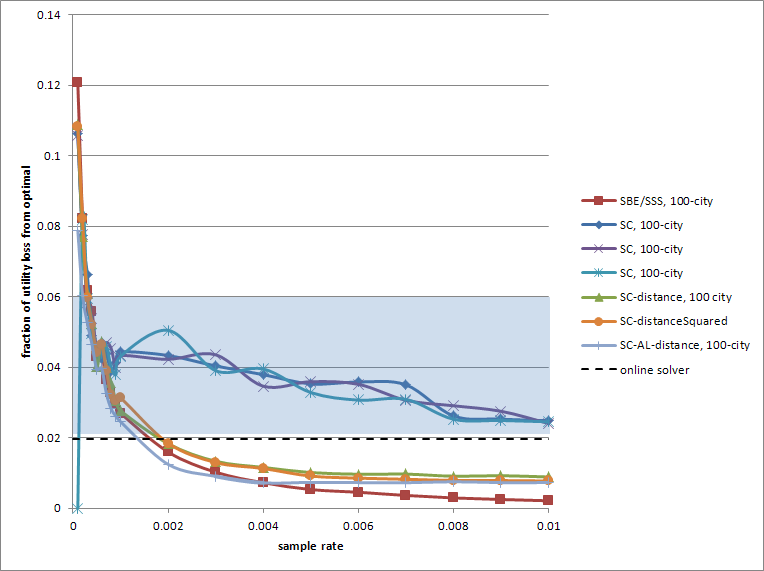
\includegraphics[scale=0.4]{pics/100tsp_baseline.eps}
\caption{Results of applying various approximation algorithms to the 100-city TSP domain.  The dotted line represents the utility loss of the online planner.  The shaded region is the expected loss of DTSP online repair algorithms as suggested by \cite{larsen2000dvrp}.}
\label{fig:100tsp_baseline}
\end{center}
\end{figure}

\subsection{SC+Bias} 

Based on the results of the SC experiments, it became apparent that the larger solution regions tended to be represented in the approximated PS Map, but smaller regions tended to disapppear.  This occurred due to the lower probability of the initial random sample choosing a problem instance in that region, resulting in either a particular region not being represented in discovered solutions or probable solutions being assigned.  One attempt to mitigate this effect was inspired by observing that within the high-quality PS Map, more rapid changes in solutions and smaller solution regions tend to exist near city locations.  The SC+bias algorithm attempts to take advantage of this observation by biasing samples towards the regions near cities.  The city radius and bias parameters determine, respectively, the radius of the region around a city to apply the bias and how much to bias the samples.  The near-city region is defined as a circle with the specified radius.  The bias represents the odds that the near-city region will be sampled.  For example, a bias value of three indicates that the near-city region will be sampled with odds 3:1 versus the non-near-city region.  

\subsubsection{Experiment Parameters} This experiment approximated a PS Map for a 100-city DTSP.  I assigned a bias factor as integers in the range from one to five, inclusive, and the city radius in the range from one to five, inclusive. The approximation algorithm was executed ten times for each combination of bias factor and city radius.

\subsubsection{Results} The results of this experiment are shown in Figures \ref{fig:scbias-results-all} and \ref{fig:scbias-results-100city-005sample}.  These results do not appear to show an obvious pattern to determine which parameters are most promising.  For example, the best performance are at the valleys (recall that lower utility loss is preferred)  at bias values of one, four, and five, and radius values of two, four, and five.  Looking at the graph, there is not an obvious gradient to suggest a generalized rule for setting these parameters.


\subsection{SC+AL} 


Sampling classification with active learning (SC+AL) is another attempt to allow for smaller solution regions to be approximated effectively.  SC+AL may be considered a generalization of SC+bias in that it allows more concentrated sampling in regions of the problem space in which the classification appears ambiguous rather than limiting the targetted samples to predetermined locations.  For example, if two solutions are both strong candidates to be assigned to a specific problem instance, then SC+AL would solve the problem instance rather than risk assigning an incorrect solution.  Similarly, if there are no strong candidates for a particular problem instance, then SC+AL would allow the problem instance to be solved rather than assign an arbitrary solution to it.  

\subsubsection{Experiment Parameters}  The alpha parameter was set to 0.5.  Thus, half of the allotted problem instances solved were selected with random sampling.  The other half were reserved for problen instances that the algorithm determines to be ambiguous.

\subsubsection{Results} The results of this experiment are shown in Figure \ref{fig:100tsp_baseline}.  At the lower sample rates, the performance of the SC+AL algorithm appears to be slightly better than the SC results.  This could suggest that at low sample rates, it is more critical to choose samples that convey the most information about the solution space.  It's reasonable that as the sample rate increases, the probability increases of obtaining that same sample information through chance.


\subsection{SSS} 

\subsubsection{Experiment Parameters}  No algorithm-specific parameters were required for this experiment.  As with the other experiments in this domain, the sample rate ranged from .0001 to .01 for a problem space consisting of 100-city DTSPs containing one variable city.

\subsubsection{Results} The results of this experiment are shown in Figure \ref{fig:100tsp_baseline}.  The utility loss of SSS quickly drops, and at sample rates greater than .003 becomes the best performing algorithm.  Intuitively, this seems reasonable:  assuming that the initial sample discovers most solutions, then testing each of the solutions against the problem instance would result in the problem instance being assigned the optimal solution.


\subsection{SBE} 

The solution border estimation algorithm (SBE) considers the mathematical features of the TSP.  It calculates the border by recognizing that the border between any two solutions is represented by equating the distance functions of the two solutions.  Unfortunately, at the time of this experiment, I did not find a Java library that could solve the complex equations that resulted from this technique.  The SBE-trace technique is inspired by SBE; however, it finds borders between two solutions by searching the space between two problem instances with known solutions.  Thus, a binary search can be employed.  Assuming that the border between two solutions is continuous, then the remainder of the border can be found by comparing the utility of the two solutions at each problem instance. 

\subsubsection{Experiment Parameters}  

No algorithm-specific parameters were required for this experiment.  As with the other experiments, the sample rate ranged from .0001 to .01 for a problem space consisting of 100-city DTSPs, with one city having variable location.

\subsubsection{Results}  The results of SBE-trace are shown in Figure \ref{fig:100tsp_baseline}.  Note that SBE-trace is only suitable for two-dimensional PS Map approximation.  Because of this limitation, it is not applicable to most domains, and thus I did not emphasize this algorithm in the subsequent experiments, which have PS Maps with higher dimenstions.


\subsection{SVM} 

The support vector machine algorithm (SVM) uses a support vector machine to try to generalize the idea of SBE to multiple dimensions.  Support vector machines calculate a maximum margin plane to separate different classes.  The observations in this application are the sampled problem instances labeled with their solutions.  

\subsubsection{Experiment Parameters}

No algorithm-specific parameters were required for this experiment.  As with the other experiments, the sample rate ranged from .0001 to .01 for a problem space consisting of 100-city DTSPs, with one city having variable location.

\subsubsection{Results}  The results of this approach are included in Figure \ref{fig:svm_svmsbe_tsp_100}.  It demonstrates that at sample rates greater than about .01, the SVM-based algorithm performs better than the online repair baseline of fractional loss of 0.02 to 0.06 as mentioned earlier.

\subsection{SVM+SBE} 

One disadvantage of the SVM-based approach is that it can misclassify problem instances.  SVM determines the borders between two solution regions by creating a margin as far as possible between known solution instances.  This process results in a border that is approximately midway between known solutions.  SVM has been shown to be a good optimization technique in general; however, it does lead to misclassifications when the actual border does not conform to this approximation.  By applying additional samples in key locations, the bounds of the margins calculated by the SVM can be made tighter and thus more consistent with the acutal borders.  In this approach, the first step is an initial set of problem instances that are sampled and solved. The second step applies the binary search used in the SBE-trace algorithm to each distinct pair of solutions, resulting in problem instances that represent solutions on the border between the distinct pair of solutions.  Finally, those problem instances and the labeled solutions are added to the training set for the SVM. 

\subsubsection{Experiment Parameters} 

The alpha parameter, which determines the fraction of the total allocated sample that will be used during random initial sampling, was set to 0.2 and 0.5.

\subsubsection{Results} The results of this approach are included in Figure \ref{fig:svm_svmsbe_tsp_100}.  It is interesting to note that the performance of SVM+SBE using an alpha value of 0.2 performs better at lower sample rates, and that with an alpha rate of 0.5 performs better at higher sample rates.  The crossover point is at a sample rate of approximately 0.02.  It appears that at higher sample rates, the random sampling is sufficient to discover the border between solutions without targetting samples.  At lower sample rates, the stucture of the solution space is not as explored, and thus it is valuable to discover key points where one solution becomes better than another.  However, at lower sample rates fewer solutions are discovered.  Thus, there is a tension between random sampling in order to discover the solutions that exist in the space, versus targetted sample which assists in accurately finding the borders between the discovered solutions.  Revisiting the SVM algorithm, which is equivalent to SVM+SBE with an alpha value of 1.0, the trend continues:  using fewer targetted samples results in worse performance at lower sample rates, but performs better at higher sample rates.




\begin{figure}
\begin{center}
\includegraphics[scale=1.0]{pics/scbias-results-all.eps}
\caption{Average utility loss of approximate PS Maps generated by SC+bias for DTSP problems of various sizes.}
\label{fig:scbias-results-all}
\end{center}
\end{figure}

\begin{figure}
\begin{center}
\includegraphics[scale=1.0]{pics/scbias-results-100city-005sample.eps}
\caption{Average utility loss of approximate PS Maps generated by SC+bias for 100-city DTSP problems at sample rate .005.  SC-generated PS Maps generated under identical conditions have an average accuracy of .035.}
\label{fig:scbias-results-100city-005sample}
\end{center}
\end{figure}


\subsection{Analysis}

These results show that these algorithms are comparable to or better than online repair performance:  all of the algorithms except for SC perform better than online repair at sample rates of .002 and above.  It is quite reasonable that the alternate algorithms would perform better than SC, because SBE and SC+AL proactively attempt to find key problem instances that distinguish one solution from another, and SSS considers more information than SC during classification.  The fact that the distance-squared version of SC performs better than the others suggests that solved problem instances that are closer to the instance being classified are more indicative of the proper solution than solved problem instances that are further away.

The results for SC+bias applied to TSP of various sizes are shown in Figure \ref{fig:scbias-results-all}.  Again, the results are comparable to online repair, but not as good as other techniques.  SC+bias has \textit{bias factor} and \textit{city radius} parameters that can be modified and were set to various values within the experiment.  Bias factor represents the degree to which to bias sampling to be near a city.  The city radius indicates how close a problem instance has to be to a city to potentially benefit from the bias.  Figure \ref{fig:scbias-results-100city-005sample} shows utility loss results at sample rate .005 when SC+bias is applied with a range of parameter configurations.  The results vary widely, and there does not appear to be any obvious correlation between specific parameter settings and the utility loss.  This behavior also appears reasonable.  The goal of this algorithm was to attempt to exploit city locations as indicators of boundaries between solution regions.  However, there are many solution regions that are not near cities; thus, this algorithm has uneven and limited benefit.

The early experiments demonstrate that SSS and SBE have the best performance.  SBE's performance is perhaps expected, as this algorithm most directly finds solution regions, thus exploiting the characteristic of this domain space in which similar problem instances tend to have similar solutions.  Alternatively, SSS's performance is best attributed to its brute-force approach of examining every problem instance and testing all known solutions.  This would seem to continue to be feasible with a tractable number of problem instances and solutions, but may not scale well.  Figure \ref{fig:sss-results-all} explores SSS and SBE's potential with additional problem sizes.  The performance continues to be good for all problem sizes, but appears to converge more rapidly for the smaller problem sizes.  This behavior is expected due to the small number of unique solutions and larger homogeneous regions.



% Not sure why these two paragraphs are here

%Results for the approximation algorithms SC, SC+AL, SSS, and SBE when applied to 100-city TSP high-quality maps are displayed in Figure \ref{fig:100tsp_baseline}.  The algorithms with ``-distance'' and ``-distanceSquared'' represent variants in which the weighting of the neighbors in the  nearest-neighbor polling is decreased as a function of the distance or distance squared from the problem take more information into account during classification.  The fact that the distance-biased versions of SC also perform better means that problem instances that are closer to the problem instance being classified are far more likely to have a similar solution than more distant problem instances.




\begin{figure}
\begin{center}
\includegraphics[scale=1.0]{pics/sss-results-all.eps}
\caption{Average utility loss of approximate PS Maps generated by SBE and SSS for DTSP problems of various sizes.}
\label{fig:sss-results-all}
\end{center}
\end{figure}



\begin{figure}
\begin{center}
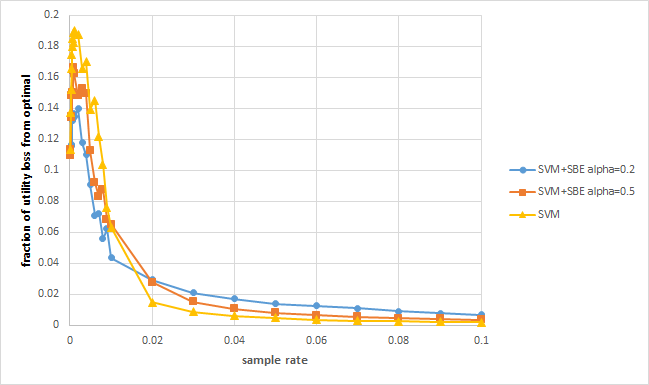
\includegraphics[scale=0.7]{pics/svm_svmsbe_tsp_100.eps}
\caption{Average utility loss of approximate PS Maps generated by SVM and SVM+SBE for 100-city TSP domain. Alpha refers to the fraction of samples used for random initial sampling.}
\label{fig:svm_svmsbe_tsp_100}
\end{center}
\end{figure}



%Focusing on the 100-city TSP as most representative of a complex domain, Figure \ref{fig:tsp-svmsbe-100city} shows the performance of SVM+SBE against a 100-city TSP high-quality PS Map for two different alpha values.  The performance is not as good as the SBE and SSS algorithms.

% source C:\Documents and Settings\holderh1\My Documents\umbc\journalPaper\pics

%\begin{figure}
%\begin{center}
%\includegraphics[scale=1.0]{pics/tsp-svmsbe-fractional-loss-vs-sample-rate.eps}
%\caption{Average utility loss of approximate PS Maps generated by SVM+SBE for 100-city DTSP problem.}
%\label{fig:tsp-svmsbe-100city}
%\end{center}
%\end{figure}




\section{Knapsack Problem}

The knapsack problem is a combinatorial optimization problem in which a subset of items of variable weight and value are chosen such that the total value is maximized and the total weight falls below  a given threshold.  For this experiment, I use the 0-1 knapsack problem variant, in which either zero or one copies of each item may be placed in the knapsack.  The knapsack is prepopulated with a set of items that utilize 396 dekagrams (dag) of the total knapsack capacity of 400 dag, and one or more items  of varying value and weight is added to the pool of items.

The knapsack domain demonstrates the applicability of the algorithms in a different domain.  One difference between this domain and the TSP domain is that it entails a more abstract representation of distance, as an item's  weight and value characteristics do not directly correspond to location and  distance as do the cities within the TSP domain. The high-quality solution PS Map's characteristics also differ in this domain.  For example, looking at the high-quality PS Map, one can see that, whereas the TSP domain had very circular homogeneous regions, the knapsack domain has rectangular homogeneous regions.  I apply the same algorithms to this domain, with the exception of the SBE-trace algorithm, which is only suitable for problem spaces of two dimensions.  I expect that performance of the algorithms could be worse in this domain, due to the greater number of solutions and smaller solution region size.



\subsection{High-Quality PS Map} For the  experiment, I defined a set of 22 items, each with known weight and value characteristics as shown in Table \ref{tab:knapsack-item-pool}, from which to maximize the value of the knapsack while conforming to its maximum weight capacity.  I defined one additional item, varying the weight and value from 1-100 inclusive to create 10,000 ($\textrm{100}^{\textrm{2}}$) problem instances.  As a baseline, I solved all 10,000 problem instances to generate a high-quality PS Map.  As with the TSP domain, I applied SSS over the PS Map to reduce errors from the heuristic solver.  A visualization of the resulting two-dimensional PS Map is depicted in Figure \ref{fig:knapsack-ideal}.

I then generated more complex problem spaces  by adding multiple items of varying weight and value characteristics to the pool.  Solving each of the resulting problem instances -- consisting of the static items and two additional items -- resulted in a four-dimensional PS Map consisting of two weight and two value dimensions.  I generated a high-quality PS Map, solving all 176,400 ($20^2 \times 21^2$) problem instances.  

Continuing, I generated an eight-dimensional problem space consisting of a weight and value axis for each of four variable items.  The range of the weight was 16 to 20 inclusive and the range of the value was 31 to 35 inclusive, resulting in a problem space of $5^8 = 390,325$ problem instances.  For each of the problem instances in the problem space, I created the full problem instance by adding the variable items indicated by the problem instance to the knapsack.  For example, if a problem instance in the problem space is $(w_0,v_0,w_1,v_1,w_2,v_2,w_3,v_3)$, then I solved a knapsack problem consisting of the pool of items in Table \ref{tab:knapsack-item-pool} plus items with weight and value scores of $(w_0,v_0),(w_1,v_1),(w_2,v_2),$ and $(w_3,v_3)$.  I solved each of the knapsack problems and created a mapping from each of the instances in the problem space to each of the calculated solution, thus composing the PS Map.

Finally, I generated a second PS Map of an eight-dimensional problem space as above, but with the range of the weight expanded by one unit to 15 to 20, resulting in a problem space of $6^4 \times 5^4 = 810,000$ instances.

\begin{figure}
\begin{center}
\includegraphics[scale=.2]{pics/knapsack-400-ideal-with-labels.eps}
\caption{High-quality PS Map for a knapsack problem.  Best viewed in color.}
\label{fig:knapsack-ideal}
\end{center}
\end{figure}

\subsection{Online Repair Baseline}  The online repair method is a greedy solver that selects the item with the highest value-to-weight ratio.


\subsection{Experiment Parameters}

The knapsack problem tested the sampling-classification (SC), sampling-classification with active learning (SC+AL), support vector machine (SVM), support vector machine with solution border estimation (SVM+SBE), and select from sampled solutions (SSS) methods.  I did not perform experiments with SBE because, as previously mentioned, it is only applicable for two-dimensional domains, and, thus, is not as useful in general cases.  The SC+Bias approximation algorithm is also omitted because its application is specific to the TSP domain's city location parameters, and there is not a clear analog within the knapsack domain.

In my experiments, I found that large regions of the problem space were homogeneous, particularly as the values of the problem instances' variable features increase.  To avoid positively skewing the results, I chose feature ranges to focus on the more heterogeneous regions of the problem instance space.  For the two-dimensional experiment, I limited the problem space to problem instances with  weights from  1-20, inclusive, and values from 50-70, inclusive.  For example, when considering only one additional item, the first problem instance would consist of the static items plus an additional item with a weight and value (1,50); the second problem would consist of the static items plus an additional item with weight and value (2,50); and so forth, accounting for all possible combinations.

The approximation of all maps was done for  sample rates ranging from .0001 to .001.  For the SC+AL and SVM+SBE algorithms, the alpha rate was set to 0.5.  Thus, the initial sample rate is half of the allocated samples, leaving half for active sampling.  As before, the evaluation of the approximation is the fraction of the utility lost with respect to the heuristically calculated heuristic solution.


\begin{table}
\begin{center}
  \begin{tabular}{|p{5cm}|p{1.5cm}|p{1.5cm}|}
    \hline
    \textbf{Object} & \textbf{Weight} & \textbf{Value} \\ \hline
    apple & 39 & 40 \\ \hline
    banana & 27 & 60 \\ \hline
    beer & 52 & 10 \\ \hline
    camera & 32 & 30 \\ \hline
    cheese & 23 & 30 \\ \hline
    compass & 13 & 35 \\ \hline
    glucose & 15 & 60 \\ \hline
    map & 9 & 150 \\ \hline
    note-case & 22 & 80 \\ \hline
    sandwich & 50 & 160 \\ \hline
    socks & 4 & 50 \\ \hline
    sunglasses & 7 & 20 \\ \hline
    suntan cream & 11 & 70 \\ \hline
    t-shirt & 24 & 15 \\ \hline
    tin & 68 & 45 \\ \hline
    towel & 18 & 12 \\ \hline
    trousers & 48 & 10 \\ \hline
    umbrella & 73 & 40 \\ \hline
    water & 153 & 200 \\ \hline
    waterproof overclothes & 43 & 75 \\ \hline
    waterproof trousers & 42 & 70 \\
    \hline
  \end{tabular}
  \caption{Knapsack static item pool}
  \label{tab:knapsack-item-pool}
\end{center}
\end{table}

\subsection{Results \& Analysis}

The result of generating a high-quality PS Map is displayed in Figure \ref{fig:knapsack-ideal}.  The map confirms an intuitive estimation of solutions: for problem instances in which the variable item's weight falls within the slack of the  original solution, it is always included in the knapsack.  Once the variable item's weight exceeds the available slack, it is excluded from the knapsack until it becomes valuable enough to replace an item currently in the knapsack.  Moving along the weight dimension, the variable item remains in the knapsack until it becomes too heavy for its value to contribute to an optimal solution and is excluded from the knapsack.  This pattern repeats, creating a set of solutions resembling a staircase of solutions, the edges of which represent a boundary in the solution space between where the variable item is included and excluded.

Figure \ref{fig:knapsack-2d-range01-loss} shows the results of applying the various PS Map approximation algorithms to a knapsack problem with one variable item.  As one might expect, most of the algorithms trend towards zero utility loss as the sample rate increases.  The notable exceptions are the SC and SSS algorithms. The SSS algorithm appears to provide somewhat of a theoretical best performance, with the other algorithms gradually converging.  The SC algorithm appears to have a much slower convergence, as it still shows a loss of approximately 20\% of the optimal utility at a 0.1 sample rate.  Figure \ref{fig:knapsack-2d-range001-loss} highlights the turbulent region up to and including sample rate 0.01.  Here it becomes apparent that the SC algorithm performs comparably to the other algorithms at this low sample rate, with the AL algorithm initially lagging behind.  Figure \ref{fig:knapsack-2d-range0001-loss} zooms in an additional time to the lower tenth of the sample rate range, up to and including 0.001, showing even more pronounced performance differences.  The SC, SVM, and SVM+SBE algorithms are generally grouped together, and the AL and SSS algorithms show a utility loss at a fairly constant level at opposite ends of the performance range.

Figures \ref{fig:knapsack-2d-range01-rank}, \ref{fig:knapsack-2d-range001-rank}, and \ref{fig:knapsack-2d-range0001-rank} show the relative rankings of the algorithms for the each of the preceding three figures.  Although the quantitative difference in performance is lost in these graphs, it does notionally illustrate the preferred algorithm as the sample rate increases.  We again see that the AL algorithms initially performs poorly, but converges quickly to become comparable to the SVM and SVM+SBE algorithms.  Conversely, the SC algorithm performance degrades and quickly becomes the worst algorithm. 

These results suggest that at very low sample rates, it is advantageous to use SC rather than AL, perhaps because SC's broader coverage of the space of problem instances is more useful than AL's targeted sampling for small sample rates.  However, at higher sample rates, the higher number of samples available for AL's initial sample appears to provide broad enough converage for the targeted sampling  to outperform the SC algorithm.  It is interesting that there is not the same level of distinction between SVM and SVM+SBE, perhaps because SVM's classifications methods permit the information gained from a sample to be applied more broadly, through the use of the maximum margin plane.  SC and AL, on the other hand, limit the use of a sample's information to a very localized region.  The advantage of SVM+SBE over SVM is that the targeted samples help to provide a more precise hyperplane location.  However, in the knapsack domain, in which the utilities of the available solutions are similar,  the benefit of the more precise hyperplane location is not as significant.  Additionally, the number of samples available for targeted sampling may not provide enough information to create a more precise margin, particularly as the number of dimensions increases.



%source C:\Documents and Settings\holderh1\My Documents\umbc\dissertation\data\k\recreateOldResults\scOutput_2011_10_01-typicalSampleRate.xlsx
%\begin{figure}
%\begin{center}
%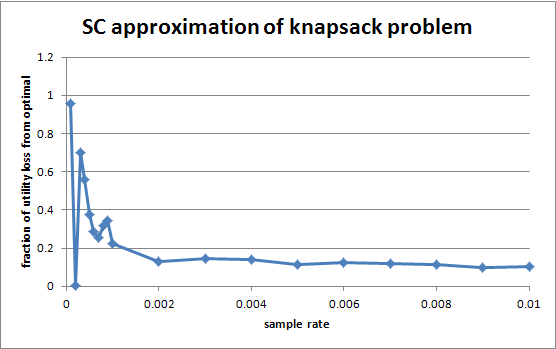
\includegraphics[scale=0.5]{pics/sc_knapsack.eps}
%\caption{SC applied to a two-dimensional knapsack problem domain.}
%\label{fig:sc_knapsack}
%\end{center}
%\end{figure}

%source C:\Documents and Settings\holderh1\My Documents\umbc\dissertation\data\recent\k_results-2d\Knapsack-2d.xlsx
%\begin{figure}
%\begin{center}
%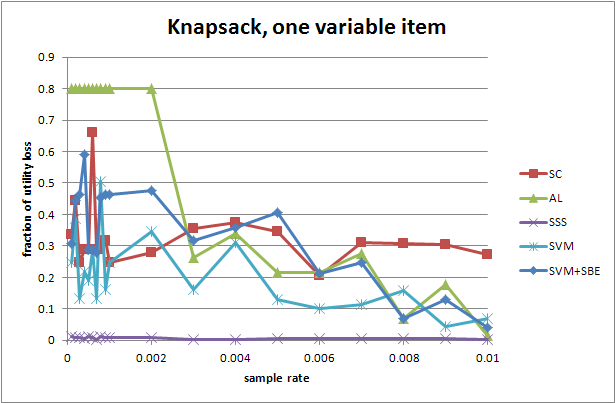
\includegraphics[scale=0.5]{pics/knapsack-2d.eps}
%\caption{Results of algorithms applied to a two-dimensional knapsack problem domain.}
%\label{fig:knapsack-2d}
%\end{center}
%\end{figure}

%C:\Documents and Settings\holderh1\My Documents\umbc\dissertation\data\recent\k_results-2d-n20-largeSampleSet/2d-n20-largeSampleSet.xlsx
\begin{figure}
\begin{center}
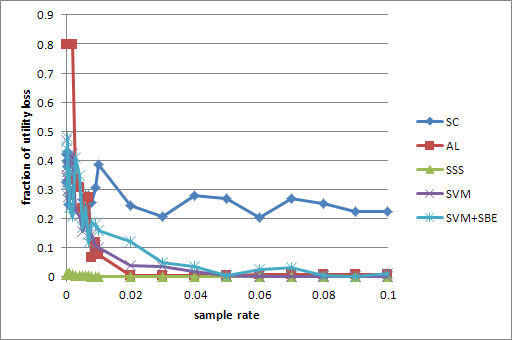
\includegraphics[scale=0.5]{pics/k-2d-n20-range01-loss.eps}
\caption{Results of algorithms applied to a two-dimensional knapsack problem domain.}
\label{fig:knapsack-2d-range01-loss}
\end{center}
\end{figure}

%C:\Documents and Settings\holderh1\My Documents\umbc\dissertation\data\recent\k_results-2d-n20-largeSampleSet/2d-n20-largeSampleSet.xlsx
\begin{figure}
\begin{center}
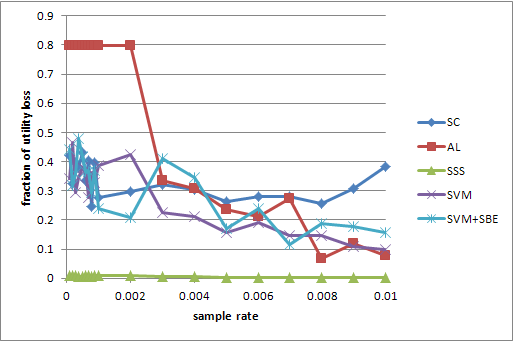
\includegraphics[scale=0.5]{pics/k-2d-n20-range001-loss.eps}
\caption{Results of algorithms applied to a two-dimensional knapsack problem domain, focus on sample rate .01 and lower.}
\label{fig:knapsack-2d-range001-loss}
\end{center}
\end{figure}

%C:\Documents and Settings\holderh1\My Documents\umbc\dissertation\data\recent\k_results-2d-n20-largeSampleSet/2d-n20-largeSampleSet.xlsx
\begin{figure}
\begin{center}
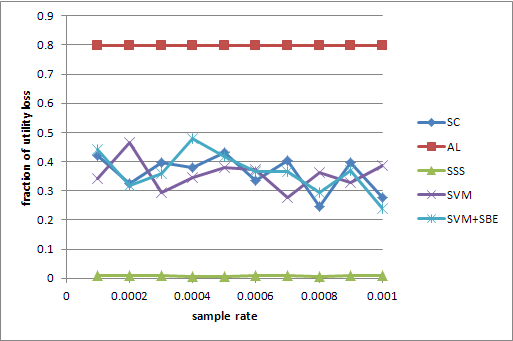
\includegraphics[scale=0.5]{pics/k-2d-n20-range0001-loss.eps}
\caption{Results of algorithms applied to a two-dimensional knapsack problem domain, focus on sample rate .001 and lower.}
\label{fig:knapsack-2d-range0001-loss}
\end{center}
\end{figure}

%C:\Documents and Settings\holderh1\My Documents\umbc\dissertation\data\recent\k_results-2d-n20-largeSampleSet/2d-n20-largeSampleSet.xlsx
\begin{figure}
\begin{center}
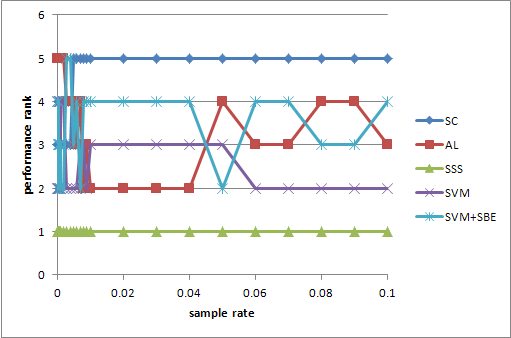
\includegraphics[scale=0.5]{pics/k-2d-n20-range01-rank.eps}
\caption{Ranking of algorithms applied to a two-dimensional knapsack problem domain.}
\label{fig:knapsack-2d-range01-rank}
\end{center}
\end{figure}


%C:\Documents and Settings\holderh1\My Documents\umbc\dissertation\data\recent\k_results-2d-n20-largeSampleSet/2d-n20-largeSampleSet.xlsx
\begin{figure}
\begin{center}
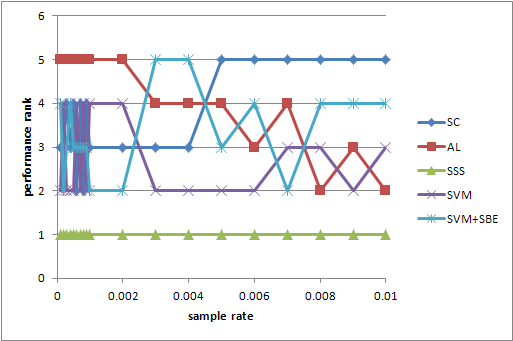
\includegraphics[scale=0.5]{pics/k-2d-n20-range001-rank.eps}
\caption{Ranking of algorithms applied to a two-dimensional knapsack problem domain, focus on sample rate .01 and lower.}
\label{fig:knapsack-2d-range001-rank}
\end{center}
\end{figure}

%C:\Documents and Settings\holderh1\My Documents\umbc\dissertation\data\recent\k_results-2d-n20-largeSampleSet/2d-n20-largeSampleSet.xlsx
\begin{figure}
\begin{center}
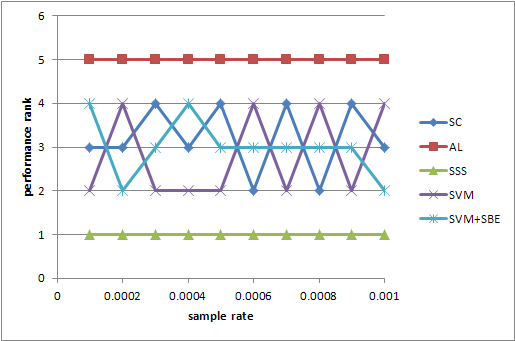
\includegraphics[scale=0.5]{pics/k-2d-n20-range0001-rank.eps}
\caption{Ranking of algorithms applied to a two-dimensional knapsack problem domain, focus on sample rate .001 and lower.}
\label{fig:knapsack-2d-range0001-rank}
\end{center}
\end{figure}

%\ref{fig:svmsbe_knapsack_4d_w14-24_v30-40}

Figure \ref{fig:knapsack-4d} shows the results of applying the PS Map approximation algorithms to a knapsack problem with two variable items.  Because each item has a weight and height characteristic, this results in a four-dimensional PS Map.  In this experiment, I limited the range of the weight and value of the items to [14,24] and [30,40], respectively, due to the computation time required to complete the experiment.  The graph shows a loss of utility well under 1\% at low sample rates.  In this domain, the algorithms appear to benefit from the higher dimensionality, because there is not a large increase in the number of unique solutions, leading to larger homogeneous solution regions that the algorithms can exploit.



The spikes in the SVM+SBE results are the effect of high variance that is a function of the manner in which SVM+SBE selects its sample points and the structure of the knapsack problem space.  After the initial random sampling, SVM+SBE uses its additional samples to find problem instances that correspond to borders between pairwise solutions. As a result, all of SVM+SBE's subsequent samples will be in a region of the problem space that is bounded by the initial sample set.  Therefore, if the initial sample does not bound a region that represents all solutions, then no subsequent samples will discover those solutions.  In this test case, the region had a total of four solutions.  If the initial sample discovered all four, then the average fraction utility loss was close to zero.  If the initial sample discovered only three solutions and none were feasible with respect to the unrepresented problem instances, then the average fraction utility loss rose to around 0.15.  If the initial sample discovered only two solutions, the average fraction utility rose to around .45, indicating that the library did not have a feasible solution for almost half of the problem instances.

This effect is less pronounced in the other algorithms.  For SC, SSS, and SVM, the probability of excluding a solution region at a particular sample rate is smaller because, unlike SVM+SBE, all of the samples are used in the initial sample, rather than a subset.  For AL, which, like SVM+SBE, also reserves a fraction of its samples for targeted sampling, its subsequent sampling targets unrepresented regions, thereby reducing the probability that a region of the problem space would remain unsampled.  The last factor is the domain, for which not all solutions are feasible for a given problem instance.  In contrast to TSP, in which any solution can be applied to any problem instance, the knapsack problem domain defines a hard constraint -- total weight -- that if  violated by a solution renders it inapplicable to the problem instance.  This characteristic leads to large losses of utility because an infeasible solution has a utility close to zero,\footnote{To avoid division-by-zero errors, the lowest utility in the knapsack problem domain is 1.} whereas in a domain like  TSP, a poor solution still does still contribute some portion of the optimal utility.


Figure \ref{fig:knapsack-4d-zoom} highlights the area of the graph where several of the algorithms appear to have similar performance.  Upon closer inspection, the typical  rapid convergence of the SSS algorithm is again visible.  In this case, the other algorithms tend asymptotically towards zero utility loss as well.


%\begin{figure}
%\begin{center}
%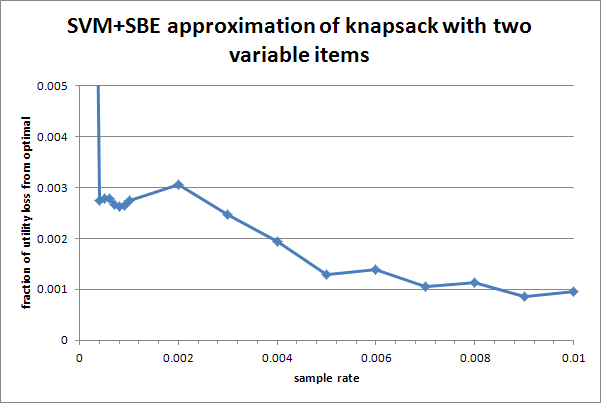
\includegraphics[scale=0.5]{pics/svmsbe_knapsack_4d_w14-24_v30-40.eps}
%\caption{SVM+SBE applied to a four-dimensional knapsack problem domain.  Problem space is limited to weight 14-24 inclusive and value 30-40 inclusive.}
%\label{fig:svmsbe_knapsack_4d_w14-24_v30-40}
%\end{center}
%\end{figure}

%C:\Documents and Settings\holderh1\My Documents\umbc\dissertation\data\recent\k_results-4d\Knapsack-4d.xlsx
\begin{figure}
\begin{center}
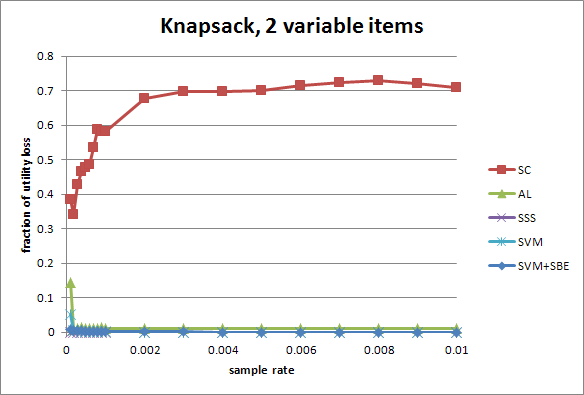
\includegraphics[scale=0.5]{pics/knapsack-4d.eps}
\caption{Results of algorithms applied to a four-dimensional knapsack problem domain.}
\label{fig:knapsack-4d}
\end{center}
\end{figure}

%C:\Documents and Settings\holderh1\My Documents\umbc\dissertation\data\recent\k_results-4d\Knapsack-4d.xlsx
\begin{figure}
\begin{center}
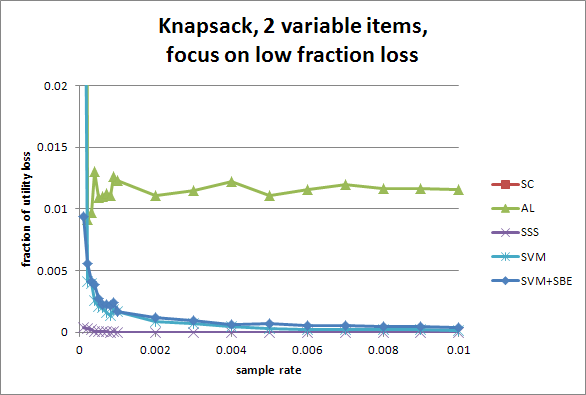
\includegraphics[scale=0.5]{pics/knapsack-4d-zoom.eps}
\caption{Results of algorithms applied to a four-dimensional knapsack problem domain, highlighting low utility loss.}
\label{fig:knapsack-4d-zoom}
\end{center}
\end{figure}


Figure \ref{fig:svmsbe_knapsack_4d_baseline} puts these results in context against various baselines.  The taller blue bars represent the fraction of utility lost if one were to assume a PS Map consisting of a single solution.  Because the high-quality PS Map had seven solutions, there are seven cases represented in the graph.  In this scheme, it is possible that the penalty for plan infeasibility could dominate the error results.  The shorter red bar represents the result of applying a default solution to a problem instance, but allows the system to choose an alternate solution if the default solution violates the weight threshold of the knapsack. In this case, a feasible plan is randomly chosen.  The upper dotted line represents the fraction of utility loss of SVM+SBE at a sample rate of .004.  The lower dotted line represents the identical loss of the online repair method as well as when sampling at a rate of .006 using SVM+SBE.  The online repair method is a greedy solver that selects the items with the highest value to weight ratios.  This demonstrates that the performance of the SVM+SBE algorithm when sampling at rate of .006 is roughly equivalent to that of the online repair technique.


%source: C:\Documents and Settings\holderh1\My Documents\umbc\dissertation\data\k\svm_4d\Results-baseline.xls
\begin{figure}
\begin{center}
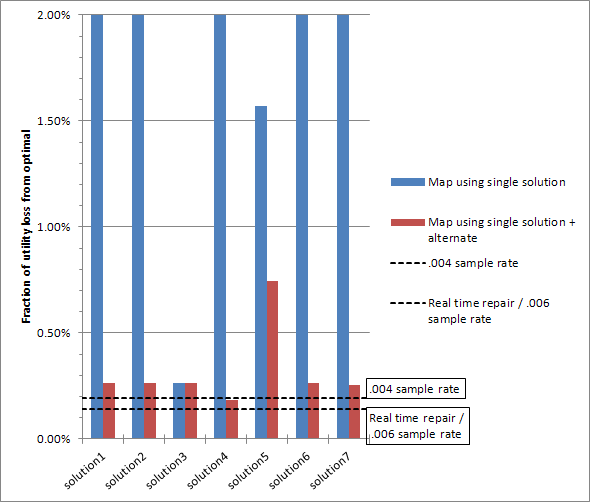
\includegraphics[scale=0.4]{pics/svmsbe_knapsack_4d_baseline.eps}
\caption{Results of applying SVM+SBE to a knapsack with two variable objects.  Dotted lines indicate fractional utility loss for online repair, .004 sample rate, and .006 sample rate, as labeled.  Bars indicate the fractional loss when using a default map consisting of either a single default solution, or a default solution and the best found feasible solution.}
\label{fig:svmsbe_knapsack_4d_baseline}
\end{center}
\end{figure}



%\begin{figure}
%\begin{center}
%\includegraphics[scale=.9]{pics/approach-results-100city.eps}
%\caption{Average utility loss of approximate PS Map generated by various approaches for 100-city DTSP problems}
%\label{fig:approach-results-100city}
%\end{center}
%\end{figure}




%\begin{figure}
%\begin{center}
%\includegraphics[scale=1.0]{pics/sss-results-all.eps}
%\caption{Average utility loss of approximate PS Maps generated by SBE and SSS for DTSP problems of various sizes}
%\label{fig:sss-results-all}
%\end{center}
%\end{figure}


\section{Elevator Problem}

The final domain, a elevator passenger transport problem,  represents a more traditional planning domain.  The TSP and knapsack domains can be considered optimization problems as well as planning problems.  The elevator domain  falls into the more traditional realm of planning, in which one has to find steps to accomplish a goal but  there is no direct mathematical representation of the domain.  Also, this domain is expected to be more challenging for the algorithms because the homogeneous regions are likely to be smaller and less regular.  Lastly, this domain represents  another level of abstraction, in that the solutions that are applied to the domain are not necessarily those that the algorithms will operate upon; the experiment parameters section describes this issue in detail.  I also apply the algorithms to this domain, again with the exception of SBE-trace.  I expect that this domain will the most challenging of the three, due to the possibility of changes in optimal plan being very sensitive to changes in the problem instance configuration.



The elevator domain is used by ICAPS in its International Planning Competition.  It specifies several elevators, floors, and passengers, and requires the planner to deliver the passengers from their starting floor to their destination floor at the lowest possible cost.  Each elevator is either ``fast'' or ``slow.''  The slow elevators incur little cost for movement, but more for stopping and starting.  Conversely, the fast elevators incur more cost for movement, but little for stopping and starting.  The planner specifies movements for the slow elevators, which may stop at any floor within a defined contiguous ``block'' of floors, and the fast elevators, which traverse the entire range of  floors, but only stop at block centers and boundaries.  For example, for a 12-floor problem with two slow elevators, one slow elevator will travel between the bottom six floors, and the other slow elevator will travel between the top six floors.  The fast elevator will travel throughout the floors, but only stop at floors 0, 3, 6, 9, and 12.  More formally, these features are specified with  M and N parameters, which create a problem domain with  M+1 total floors in blocks of N+1 floors, with fast elevators that may stop at floors that are multiples of $\frac{N}{2}$.  Thus, in the example above, M is 12 (13 floors from 0 to 12) and N is 6 (two blocks each of seven floors, one from 0 to 6 inclusive, the other from 6 to 12 inclusive).  

Typically, each planner submitted to the competition targets either the ``optimal'' or ``sacrificing'' track. The ``optimal'' track requires a planner to find the least costly means of transporting the passengers to their destinations.  The ``sacrificing'' track does not require a planner to find the optimal plan, but only to find a feasible plan to deliver all of the passengers.  My experiments focused on the optimal track and used one of the more successful planners, the LAMA Planner \citep{richter2010lama}.

\subsection{High-quality PS Map generation}  For this domain, I generated a 12-floor and two 24-floor elevator problems.  The 12-floor problem contained two seven-floor blocks (M=12, N=6), two slow elevators, and one fast elevator.  Each problem assumed two passengers with variable starting position, creating 169 problems to be solved with the LAMA planner.  One 24-floor configuation consisted of six five-floor blocks (M=24, N=4), and the other contained four seven-floor blocks (M=24, N=6).  The 24-floor problems vary the starting location of three passengers, thereby creating a high-quality map of 216 (i.e., $6^3$) problem instances.


Similar to other hard problems, planners in this domain employ heuristics in order to solve these intractable problems, and thereby benefit from ``smoothing'' as described in Section \ref{sec:sss}:  when generating the high-quality PS Map, each of the solutions is evaluated against each of the problem instances, and, if necessary, the problem instance is assigned a new solution.  This prevents the odd phenomenon of the occasional approximate solution having better utility than the ``optimal'' solution, which may skew the results.

\subsection{Experiment Parameters} My initial experiment used the 12-floor problem with three passengers, two slow elevators, and one fast elevator.  I varied the starting positions of two passengers, resulting in a 169-instance problem space.  In my initial experiment, there were too many unique plans, and the algorithms could not create classifications from the sampling. To make this domain appropriate for the algorithm, I abstracted the plans to transform a plan that moves elevators to a specific floor into a plan to move elevators to the location of specific passengers, thus creating a plan that could be applied to other problem instances.  For example, consider a raw plan with the steps

\begin{verbatim}
(move-down-slow slow0-0 n6 n0)
(board p0 slow0-0 n0 n0 n1)
(move-up-slow slow0-0 n0 n3)
(leave p0 slow0-0 n3 n1 n0)
\end{verbatim}

\noindent
This plan specifies that, first, the slow elevator with id slow0-0 moves from floor 6 to floor 0.  Next, the passenger with id p0 boards the elevator at floor 0, and the number of passengers increases from 0 to 1.  Then the elevator moves from floor 0 to floor 3, and in the final step, the passenger leaves the elevator at floor 3 and the number of passengers in the elevator decreases from 0 to 1.

In order to make this plan reusable, it is transformed to be  more general:

\begin{verbatim}
elevator slow0-0 picks up passenger p0
elevator slow0-0 drops off passenger p0
\end{verbatim}

The first step specifies that the elevator with id slow0-0 moves to passenger p0's current location, and p0 boards the elevator.  The second step then specifies that the elevator moves to passenger's desired destination and the passenger disembarks.  This general plan can  be applied to problem instances in which the elevator and passengers are on floors other than those assumed by the raw plan.

In addition to abstracting the plans, I normalize the plan so that differences in the ordering of independent actions are not interpreted as distinct plans.  For example, consider the plan below, annotated with action ids for ease of reference: 

\begin{verbatim}
1: elevator slow0-0 picks up passenger p0
2: elevator slow1-0 picks up passenger p1
3: elevator slow0-0 drops off passenger p0
4: elevator slow1-0 drops off passenger p1
\end{verbatim}

Note that the only dependencies are that action 1 must occur before action 3, and action 2 must occur before action 4.  Thus, there are six potential plans\footnote{(1,2,3,4), (1,2,4,3), (1,3,2,4), (2,1,3,4), (2,1,4,3), and (2,4,1,3)} representing the same overall process.  I normalize the plan by grouping together as many actions as possible that are performed by the same elevator.  In this case, the resulting normalization is:

\begin{verbatim}
1: elevator slow0-0 picks up passenger p0
3: elevator slow0-0 drops off passenger p0
2: elevator slow1-0 picks up passenger p1
4: elevator slow1-0 drops off passenger p1
\end{verbatim}

My subsequent experiments used a 24-floor elevator problem with six passengers, three of which had variable starting locations.  One experiment used six fast elevators and three slow elevators, and the other used four slow elevators.

\subsection{Online Repair Baseline} As a baseline, I implemented an online repair algorithm.  \cite{krogt05planrepair} describe plan repair as consisting of removing actions from the original plan that conflict with or impede achieving the new goal, followed by adding actions to the original plan that allow it to achieve the new goal.  My baseline online replanning algorithm is consistent with this methodology.  The new goal changes the initial location of the passenger, and thus I consider all actions that reference that passenger as candidates for deletion.  \citeauthor{krogt05planrepair} suggest that heuristics should be used to determine if a candidate action should be deleted.  My  heuristic is a simple one: I only remove the candidate action if it refers to a passenger whose starting position has moved outside the range of the elevator used by  the action.  For example, consider an abstracted action \textit{elevator slow0-0 picks up passenger p0}. Elevator slow0-0's range is floors n0 through n6. If this action is applied to a problem instance in which p0's starting position is n7 or above, then the action would be removed.

% TODO need a concrete example to clarify
In the event that an action is removed, I proceed with the second component of plan repair, in which I add actions to the original plan to achieve the new goal.  There are two alternatives for continuation:  either remove all subsequent actions that refer to the passenger and replan the entire route, or preserve the subsequent actions and replan the passenger route to comply with the constraints implied by the subsequent actions.  In the case of the former, I generate a solution to transport the passengers whose actions were removed.  In order to plan without the influence of the passengers whose actions have already been established, the initial starting conditions of those passengers is set to be equal to their destination location.  In the case of the latter, the final condition is set to the location expected by the action that moves the passenger to its final destination.  For example, if an action moves p2 from n6 to n2 to complete its journey, then the planner will set the final destination to n6.


\begin{algorithm}
%\caption{unrefinement strategy $<\mathcal{P},\mathcal{H}'> = \mathcal{D}(P,\mathcal{H})$\\Input: plan P and history $\mathcal{H}$\\Output: plan set $\mathcal{P}$ and updated history $\mathcal{H}'$}
\caption{Unrefinement}
\label{alg:p}

%\small
\begin{algorithmic}[1] 
  
  \For{each passenger p in plan P}
    \If{first action referencing p is invalid}
      \State remove all actions referencing p
    \EndIf
  \EndFor

\end{algorithmic}
\end{algorithm}


\begin{algorithm}
%\caption{refinement strategy $<\mathcal{P},\mathcal{H}'> = \mathcal{R}(P,\mathcal{H})$\\Input: plan P and history $\mathcal{H}$\\Output: plan set $\mathcal{P}$ and updated history $\mathcal{H}'$}
\caption{Refinement}
\label{alg:r}

%\small
\begin{algorithmic}[1] 
  \State {actions} $\leftarrow$ generate plan for deleted passenger actions
  \State parse and abstract {actions}
  \State add {actions} to P
  \State normalize P
\end{algorithmic}
\end{algorithm}


% I found that even with these plans, there were still too many distinct plans to allow SVM+SBE processing to be effective. I moved to a 24-floor problem instance in the hope that there would be larger regions of homogeneous plans that the SVM+SBE algorithm would be able to take advantage of.

%The 24-floor plan did not fit the constraints of the typical elevator domain problem, but this did not affect the planners.  It may have been an issue if were automatically generating the problem definition files, but I modified those by hand.

\subsection{Results}

Results from the 12-floor elevator problem domain are displayed in Figure \ref{fig:svmsbe_elevator_12}.  The dotted lines represent the fractional utility loss of three independent runs of the online repair algorithm described in Algorithms \ref{alg:p} and \ref{alg:r}.  The solid lines represent the results of applying the SVM+SBE approximation algorithm with various SVM kernels and the SSS algorithm.  The results demonstrate that the SSS algorithm has less fractional utility loss than the online algorithms, but the various SVM+SBE algorithms generally perform worse than the online repair algorithms.


Figures \ref{fig:elevator-3pass-maxsample05} through \ref{fig:elevator-3pass-maxsample001} show results of all the algorithms applied to the same 12-floor configuration mentioned above.  Again, the utility loss is much greater in this domain than in other domains.  This is due to the small number of unique solutions and the smaller size of homogeneous regions in the space.  This effect can be observed more explicitly by examining the performance of the algorithms in two different 24-floor configurations.  


%source:  C:\Documents and Settings\holderh1\My Documents\umbc\dissertation\lamaPlanner\work\p01-3d\results\svmElevatorOutput3D_2013_11_05__19_06_27-p01_3d-normalization.xlsx
%\begin{landscape}
\begin{figure}
\begin{center}
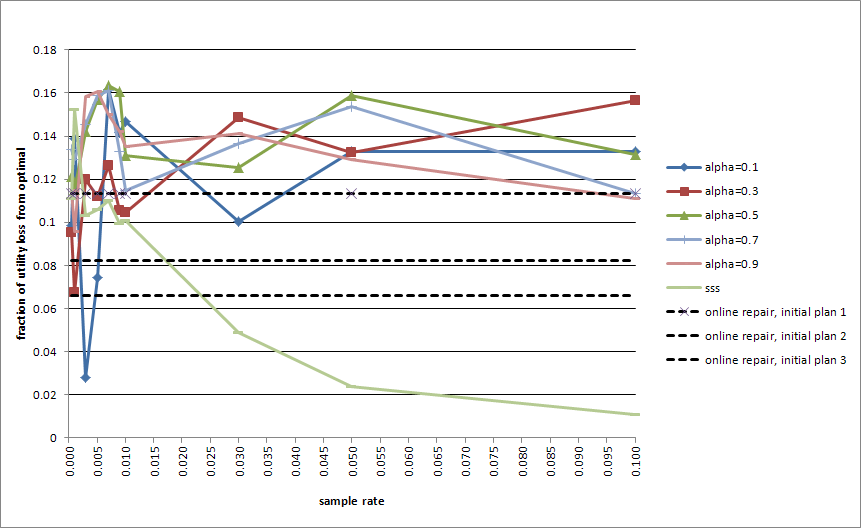
\includegraphics[scale=.5]{pics/svmsbe_elevator_12.eps}
\caption{Results of applying the SVM+SBE algorithm to a 12-floor elevator problem consisting of 2 slow elevators, 1 fast elevator, and 3 variable passenger starting locations.  Dotted lines represent the utility loss of online repair.  Solid lines represent approximations using various alpha values.}
\label{fig:svmsbe_elevator_12}
\end{center}
\end{figure}
%\end{landscape}




%source:     dissertation/lamaPlanner/work/p01-3d/results/nov8
\begin{figure}
\begin{center}
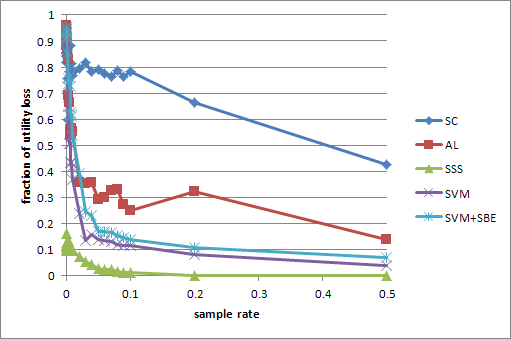
\includegraphics[scale=.5]{pics/elevator-3pass-maxsample05.eps}
\caption{Results of applying various approximation algorithms to a 12-floor elevator problem consisting of 2 slow elevators, 1 fast elevator, and 3 variable passenger starting locations.}
\label{fig:elevator-3pass-maxsample05}
\end{center}
\end{figure}

\begin{figure}
\begin{center}
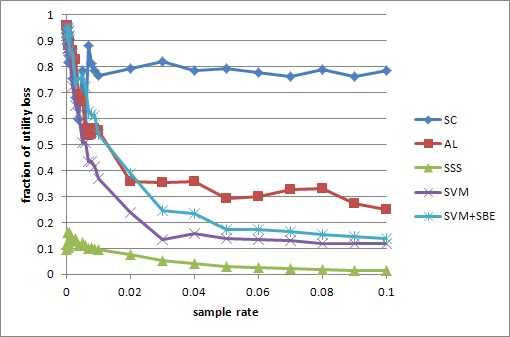
\includegraphics[scale=.5]{pics/elevator-3pass-maxsample01.eps}
\caption{Results of applying various approximation algorithms to a 12-floor elevator problem consisting of 2 slow elevators, 1 fast elevator, and 3 variable passenger starting locations, focus on sample rate 0.1 and lower.}
\label{fig:elevator-3pass-maxsample01}
\end{center}
\end{figure}

\begin{figure}
\begin{center}
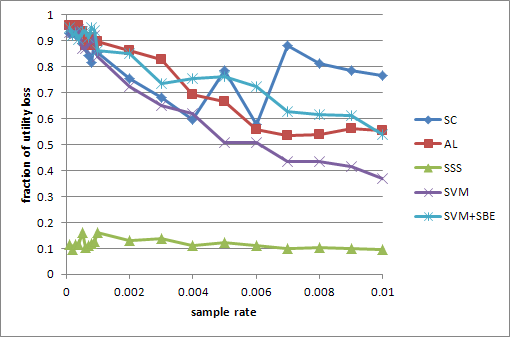
\includegraphics[scale=.5]{pics/elevator-3pass-maxsample001.eps}
\caption{Results of applying various approximation algorithms to a 12-floor elevator problem consisting of 2 slow elevators, 1 fast elevator, and 3 variable passenger starting locations, focus on sample rate 0.01 and lower.}
\label{fig:elevator-3pass-maxsample001}
\end{center}
\end{figure}





Results from the 24-floor elevator domain experiments are shown in Figures \ref{fig:elevator-6pass-maxsample05} through \ref{fig:elevator-6pass-nofast-maxsample001}.  These results show that for each problem configuration, SSS performs better than SVM+SBE.  Additionally, the algorithms perform better against the problem configuration with fewer elevators.  This is not unexpected,  given the nature of the problem space of each configuration and the algorithms used.  In all of the configurations, the problem spaces have homogeneous regions, but they are small, which can make it difficult for an SVM-based algorithm to converge and find the appropriate boundaries.  However, those small regions are not a disadvantage for the SSS algorithm, because it chooses a solution for each unsolved problem instance, rather than attempting to find groupings like SVM+SBE.  This same logic is applicable to the generally better results for the problem configuration with fewer elevators.  In the  configuration with four slow elevators, the homogeneous regions are larger than in the  problem space with six slow elevators, and thus the SVM+SBE algorithm performs better.  Because there are fewer total solutions in the configuration with fewer elevators, the SSS algorithm performs better as well.





\begin{figure}
\begin{center}
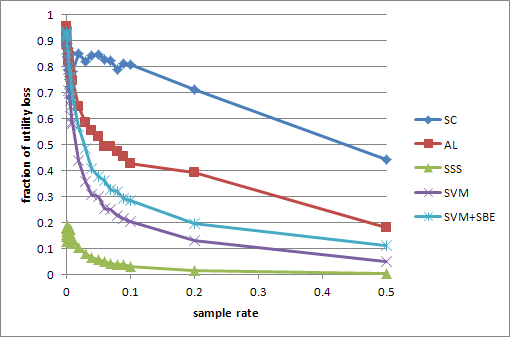
\includegraphics[scale=.6]{pics/elevator-6pass-maxsample05.eps}
\caption{Results of applying various approximation algorithms to a 24-floor elevator problem consisting of 6 slow elevators, 3 fast elevators, and 3 variable passenger starting locations of 6 total.}
\label{fig:elevator-6pass-maxsample05}
\end{center}
\end{figure}

\begin{figure}
\begin{center}
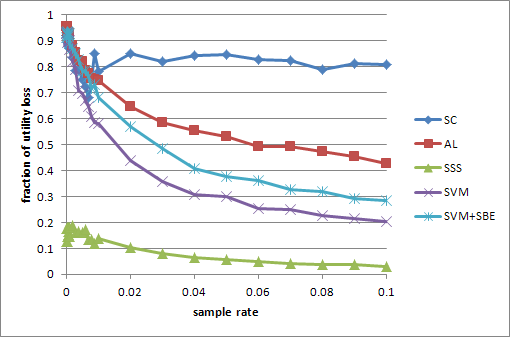
\includegraphics[scale=.6]{pics/elevator-6pass-maxsample01.eps}
\caption{Results of applying various approximation algorithms to a 24-floor elevator problem consisting of 6 slow elevators, 3 fast elevators, and 3 variable passenger starting locations of 6 total, focus on sample rate 0.1 and lower.}
\label{fig:elevator-6pass-maxsample01}
\end{center}
\end{figure}

\begin{figure}
\begin{center}
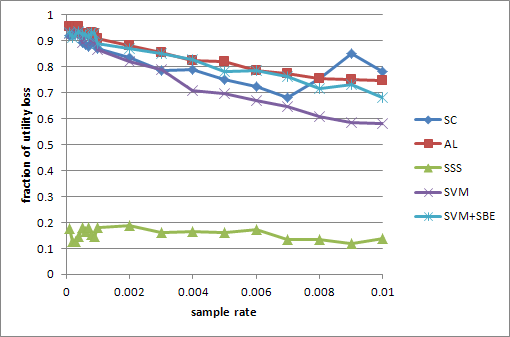
\includegraphics[scale=.6]{pics/elevator-6pass-maxsample001.eps}
\caption{Results of applying various approximation algorithms to a 24-floor elevator problem consisting of 6 slow elevators, 3 fast elevators, and 3 variable passenger starting locations of 6 total, focus on sample rate 0.01 and lower.}
\label{fig:elevator-6pass-maxsample001}
\end{center}
\end{figure}






%sources:  dissertation/lamaPlanner/work/p-6pass/results/nov8
%          dissertation/lamaPlanner/work/p-6pass-nofast/results/nov8
%          dissertation/lamaPlanner/work/p01-3d/results/nov8
\begin{figure}
\begin{center}
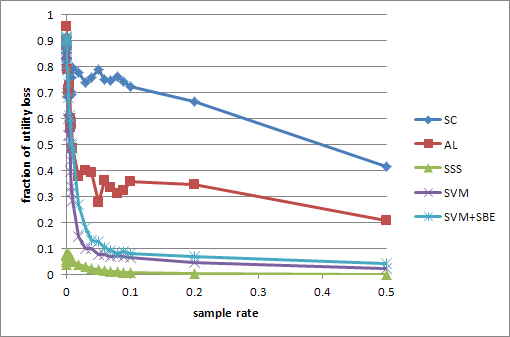
\includegraphics[scale=.6]{pics/elevator-6pass-nofast-maxsample05.eps}
\caption{Results of applying various approximation algorithms to a 24-floor elevator problem consisting of 4 slow elevators, 0 fast elevators, and 3 variable passenger starting locations of 6 total.}
\label{fig:elevator-6pass-nofast-maxsample05}
\end{center}
\end{figure}


\begin{figure}
\begin{center}
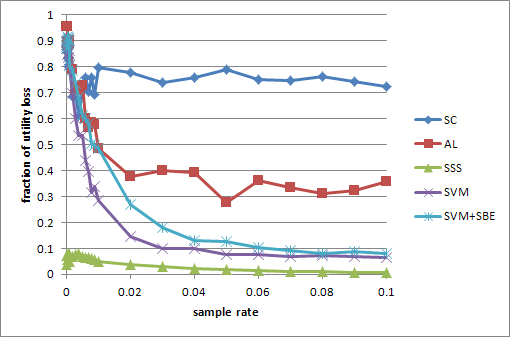
\includegraphics[scale=.6]{pics/elevator-6pass-nofast-maxsample01.eps}
\caption{Results of applying various approximation algorithms to a 24-floor elevator problem consisting of 4 slow elevators, 0 fast elevators, and 3 variable passenger starting locations of 6 total, focus on sample rate 0.1 and lower.}
\label{fig:elevator-6pass-nofast-maxsample01}
\end{center}
\end{figure}

\begin{figure}
\begin{center}
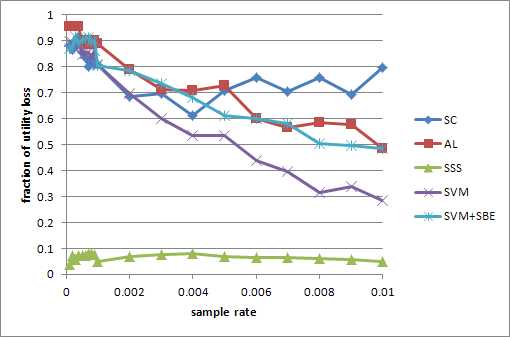
\includegraphics[scale=.6]{pics/elevator-6pass-nofast-maxsample001.eps}
\caption{Results of applying various approximation algorithms to a 24-floor elevator problem consisting of 4 slow elevators, 0 fast elevators, and 3 variable passenger starting locations of 6 total, focus on sample rate 0.01 and lower.}
\label{fig:elevator-6pass-nofast-maxsample001}
\end{center}
\end{figure}

%\begin{figure}
%\begin{center}
%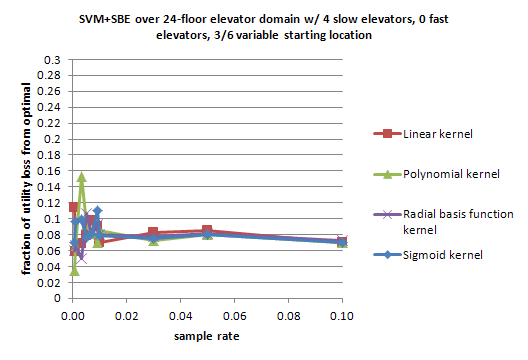
\includegraphics[scale=.6]{pics/svmsbe_elevator_4slow_0fast_6pass_3d.eps}
%\caption{Results of applying the SVM+SBE algorithm to a 24-floor elevator problem consisting of 4 slow elevators, 6 passengers, and 3 variable passenger starting locations.}
%\label{fig:svmsbe_elevator_4slow_0fast_6pass_3d}
%\end{center}
%\end{figure}



%\begin{figure}
%\begin{center}
%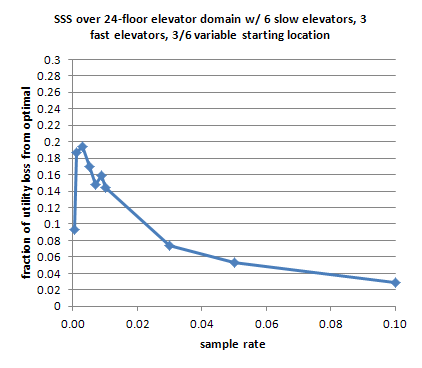
\includegraphics[scale=.6]{pics/sss_elevator_6slow_3fast_6pass_3d.eps}
%\caption{Results of applying the SSS algorithm to a 24-floor elevator problem consisting of 6 slow elevators, 3 fast elevators, 6 passengers, and 3 variable passenger starting locations.}
%\label{fig:sss_elevator_6slow_3fast_6pass_3d}
%\end{center}
%\end{figure}

%\begin{figure}
%\begin{center}
%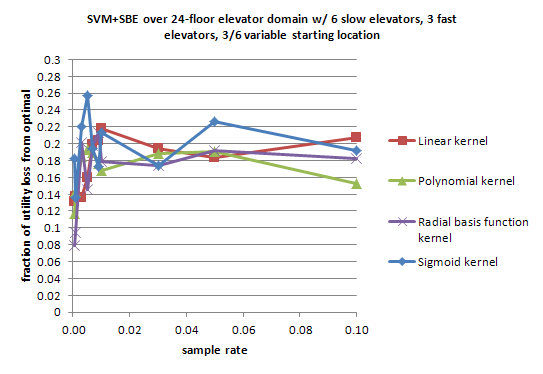
\includegraphics[scale=.6]{pics/svmsbe_elevator_6slow_3fast_6pass_3d.eps}
%\caption{Results of applying the SVM+SBE algorithm to a 24-floor elevator problem consisting of 6 slow elevators, 3 fast elevators, 6 passengers, and 3 variable passenger starting locations.}
%\label{fig:svmsbe_elevator_6slow_3fast_6pass_3d.eps}
%\end{center}
%\end{figure}


\section{Overall Analysis \& Discussion}

The results generally show little difference between approaches at low sample rates.  In fact, the results tend to be highly volatile, perhaps due to the high dependence on a small number of samples, which leads to large variances in the solutions available for the algorithms to consider.

SC tends to be a reasonable approach, with the added benefit that it is very simple to implement.  SC+bias shows the ability to improve on SC; however, it is not clear how to tune its parameters to achieve consistently good results.  SBE clearly is the best performer in the domains in which it was applied.  However, my implementation of SBE is limited to two dimensions.  SSS tends to have  the same results as SBE, but SSS is more computationally intensive, potentially leading to scaling issues in large problem spaces.  

The use of the SVM approach was intended to mimic the idea of SBE, but adds the ability to apply it higher-dimensional domains.  This approach tended to yield reasonable results.  Augmenting SVM with additional points to constrain the margin plane in SVM+SBE did not appear to have the significant impact one might have expected.  This may be because the test domains are fairly forgiving when applying a less optimal solution to a problem instance.  A domain in which there is a larger penalty for less optimal solutions may require an approach like SVM+SBE, which would provide a more accurate classification of solutions to the problem instances.  Although SVM and SVM+SBE did not achieve the results of SSS or SBE, they do have the advantage of being less computationally intensive and being applicable to domains of more than two dimensions.

The results of all algorithms appear to be sensitive to problem domain characteristics.  In the case of TSP, for example, larger size and a smaller quantity of homogeneous solutions regions generally resulted in better performance by the algorithms. This was also apparent when comparing the performance of the algorithms in the various elevator domain configurations.  The algorithms were able to perform well when tested against configurations that resulted in large homogeneous spaces in the solution space.

Most importantly, the results do demonstrate that these techniques are useful as an alternative to online plan repair.  At the appropriate sample rate, performance tends to be comparable, and sometimes better, than the online solution.  The benefit of my approach is that, assuming the ability to compute the necessary library before the environment changes, the new plan can be accessed much more rapidly than the online repairer can calculate a new plan.  These tradeoffs are discussed in more detail in the next chapter.

